% template.tex
% 서강대학교 AI·SW대학원 석사학위논문 LaTeX 템플릿
%
% 본 문서는 작성 가이드 겸 템플릿입니다.
% 내용을 본인 논문으로 바꾸기 전에, 먼저 전체 구성을 읽어 보시기 바랍니다.
% 한글 조판용 패키지(kotex)가 설치된 TeX 배포판이 필요합니다.
%
\documentclass[korean]{aisw}

% 필요 시 추가 패키지를 여기에 넣습니다.
\usepackage{graphicx}
\usepackage{booktabs}
\usepackage{verbatim}

%------------------------------------------------------------------------------
% 제목·저자·날짜 등 — 본인 정보로 교체합니다.
%------------------------------------------------------------------------------
\title[korean]{서강대학교 AI\textbullet SW대학원 \\ 학위논문 \LaTeX\ 작성 가이드}
\title[english]{A \LaTeX\ Writing Guide for Master's Theses \\ at the Graduate School of AI\textbullet SW, Sogang University}

\author[korean]{김 석 사} % 반드시 한 칸씩 띄어쓰기할 것
\author[english]{Seoksa Kim}
\author[nospace]{김석사} % 공백 없는 한글 이름

\adviser{김 지 도}

\major[korean]{데이터사이언스 \textbullet\ 인공지능 전공}
\major[english]{MAJOR OF DATA SCIENCE \textbullet ARTIFICIAL INTELLIGENCE}

\committeememberA{김 주 심}
\committeememberB{김 지 도}
\committeememberC{김 부 심}

\submissiondeadline{20XX년 X월 X일}
\examinationdate{20XX년 X월 X일}
\gradyear[english]{June 20XX}
\gradyear[korean]{20XX년 6월}

% 장-절 번호 체계 (필요에 따라 유지·수정합니다.)
\setcounter{secnumdepth}{3}
\renewcommand\thechapter{\arabic{chapter}}
\renewcommand\thesection{\arabic{chapter}.\arabic{section}}
\renewcommand\thesubsection{(\arabic{subsection})}
\renewcommand\thesubsubsection{(\gana{subsubsection})}

\begin{document}
\renewcommand{\baselinestretch}{1.6}    % 본문 줄간격(지침 160\%--200\%). 고치지 않는 것을 권장합니다.
\selectfont

\acknowledgement{
    \par
    본 문서는 서강대학교 AI\textbullet SW대학원 석사 학위논문 작성을 위한
    \LaTeX\ 작성 가이드 겸 템플릿입니다.
    표지·인준서·초록·본문·참고문헌의 형식을 확인하신 뒤,
    제목·이름·본문을 논문 작성자의 연구 내용으로 교체하여 사용하시기 바랍니다.
}

\newpage
\makelists

\begin{summary}
    \par
    This document is both an instruction guide and a working template for
    master's theses at the Graduate School of AI\textbullet SW, Sogang University.
    It demonstrates how to set the title, author, and other fields, structure chapters and sections,
    insert tables and figures, write equations, and cite references with
    \texttt{aisw.cls}, \texttt{aisw.bst}, and \texttt{mybib.bib}.
    Replace the placeholder content with your own research before submission.
    \vfill
    \begin{minipage}[t][20mm][b]{\textwidth}
        {\bfseries keywords}: \LaTeX, thesis template, Sogang University, AI\textbullet SW\\
    \end{minipage}
\end{summary}

\newpage

\begin{abstract}
    \par
    본 문서는 서강대학교 AI\textbullet SW대학원 석사 학위논문용
    \LaTeX\ 작성 가이드 겸 템플릿입니다.
    \texttt{aisw.cls}와 \texttt{aisw.bst}, \texttt{mybib.bib}를 사용하여
    표지·인준서·초록·장절 구성·표·그림·수식·참고문헌을 작성하는 방법을 안내합니다.
    제출 전에는 예시로 넣은 제목·이름·본문을 논문 작성자의 연구 내용으로 모두 교체하시기 바랍니다.
    \vfill
    \begin{minipage}[t][20mm][b]{\textwidth}
        {\bfseries 키워드}: \LaTeX, 학위논문, 템플릿, 서강대학교, AI\textbullet SW\\
    \end{minipage}
\end{abstract}

%==============================================================================
\chapter{환경 설정}
%==============================================================================

\section{본 템플릿의 사용 방법}

권장 작업 순서는 다음과 같습니다.
\begin{enumerate}
    \item 본 문서를 끝까지 읽어 형식과 빌드 방법을 파악합니다.
    \item \texttt{template.tex}를 복사하여 \texttt{mythesis.tex} 등으로 이름을 바꿉니다.
    \item 제목·저자·지도교수·심사위원·날짜 등 정보를 수정합니다.
    \item 본문·표·그림·참고문헌을 교체합니다.
    \item 아래 빌드 순서로 PDF를 확인한 뒤 제출합니다.
\end{enumerate}

\section{운영체제별 \LaTeX\ 설치}

한국어 문서 작성을 위해 \texttt{kotex}가 포함된 배포판을 설치합니다.
\texttt{.tex} 파일을 편집한 뒤, 아래 빌드 명령으로 PDF를 만들면 됩니다.

\subsection{Windows}

Windows에서는 \textbf{TeX Live}를 권장합니다.
\begin{enumerate}
    \item \url{https://tug.org/texlive/}에서 Windows용 설치 프로그램을 받습니다.
    \item \texttt{install-tl-windows.bat}를 실행하여 설치합니다. (전체 scheme 권장)
\end{enumerate}
대안으로 MiKTeX(\url{https://miktex.org/})를 사용할 수 있습니다.
MiKTeX는 필요한 패키지를 컴파일 시 자동으로 내려받습니다.

\subsection{macOS}

macOS에서는 \textbf{MacTeX}를 권장합니다.
\url{https://tug.org/mactex/}에서 \texttt{.pkg}를 받아 설치합니다.

\subsection{Linux}

Ubuntu/Debian 계열에서는 다음을 권장합니다.
\begin{verbatim}
sudo apt update
sudo apt install texlive-full
\end{verbatim}
용량을 줄이려면 \texttt{texlive-lang-korean} 등 필요한 패키지만 설치할 수 있습니다.
패키지 추가는 \texttt{tlmgr}를 사용합니다.

\subsection{Overleaf}

Overleaf를 사용하는 경우, 프로젝트에 \texttt{aisw.cls}, \texttt{aisw.bst},
\texttt{mybib.bib}, \texttt{figures/}를 함께 업로드하고
메인 파일을 \texttt{template.tex}(또는 본인 \texttt{.tex})로 지정합니다.
컴파일러는 \textbf{pdfLaTeX}로 설정합니다.

\section{빌드 방법}

참고문헌을 포함한 완전한 PDF를 만들려면 다음 순서를 따릅니다.

\begin{verbatim}
pdflatex template
bibtex template
pdflatex template
pdflatex template
\end{verbatim}

\begin{enumerate}
    \item 1단계(\texttt{pdflatex}): 인용 정보를 모아 \texttt{.aux}를 만듭니다.
    \item 2단계(\texttt{bibtex}): \texttt{mybib.bib}에서 항목을 가져와 서식을 적용합니다.
    \item 3--4단계(\texttt{pdflatex}): 참고문헌·인용 번호·목차를 반영합니다.
\end{enumerate}

%==============================================================================
\chapter{문서 구조와 표지}
%==============================================================================

\section{자동 생성되는 앞부분}

문서 맨 위에 제목·저자 등을 채운 뒤 빌드하면
겉표지·속표지·제출문·인준서가 자동으로 생성됩니다.
이어서 감사의 뜻(\texttt{\textbackslash acknowledgement\{\}}),
차례(\texttt{\textbackslash makelists}),
영문 초록(\texttt{summary}), 국문 초록(\texttt{abstract}) 순으로 작성합니다.

학위논문작성지침~\cite{sogang2025aiswthesisguide}에 따른 순서는 다음과 같습니다.

\textbf{겉표지 -- 속표지 -- 제출문 -- 인준서 -- 감사의 뜻 -- 차례 --
표 차례 -- 그림 차례 -- 초록 -- 본문 -- 참고문헌}

본문의 줄간격은 지침상 160\%--200\%이므로, 본 템플릿은
\texttt{\textbackslash baselinestretch\{1.6\}}을 기본으로 둡니다.
행간이 너무 좁으면 값을 올려 가며 확인하시기 바랍니다. (상한 2.0)

\section{문서 맨 위에서 반드시 채울 항목}

\begin{itemize}
    \item \texttt{\textbackslash title[korean/english]} — 국문·영문 제목
    \item \texttt{\textbackslash author[korean/english/nospace]} —
          한국어는 띄어쓴 이름과 붙여 쓴 이름을 모두 넣습니다.
    \item \texttt{\textbackslash adviser} — 지도교수(한국어)
    \item \texttt{\textbackslash major[korean/english]} — 전공
    \item \texttt{\textbackslash committeememberA/B/C} — 심사위원
    \item \texttt{\textbackslash submissiondeadline},
          \texttt{\textbackslash examinationdate} — 제출일·심사일
    \item \texttt{\textbackslash gradyear[korean/english]} — 표지용 졸업년월
          (예: \texttt{2026년 6월} / \texttt{June 2026})
\end{itemize}

%==============================================================================
\chapter{장·절·항·목 작성}
%==============================================================================

\section{계층 구조}\label{sec:heading}

본 템플릿의 본문 계층은 다음과 같습니다.
학위논문작성지침의 「장--절--(1)--(가)」 구분과 같습니다.

\begin{itemize}
    \item \texttt{\textbackslash chapter\{...\}} — 장
    \item \texttt{\textbackslash section\{...\}} — 절
    \item \texttt{\textbackslash subsection\{...\}} — 항
    \item \texttt{\textbackslash subsubsection\{...\}} — 목
\end{itemize}

현재 번호 체계는 장~\arabic{chapter},
절~\ref{sec:heading}과 같이
\texttt{장.절}, 항은 \texttt{(1)}, 목은 가나다 표기를 사용합니다.
\texttt{subsubsection}(목)은 차례에 나타나지 않도록 설정되어 있습니다.

\subsection{항 예시}

이 문단은 \texttt{\textbackslash subsection}(항)의 표시 예시입니다.

\subsubsection{목 예시}

이 문단은 \texttt{\textbackslash subsubsection}(목)의 표시 예시입니다.

\section{상호 참조}

\texttt{\textbackslash label}과 \texttt{\textbackslash ref},
\texttt{\textbackslash eqref}, \texttt{\textbackslash cite}를 사용하면
항목을 추가해도 번호를 직접 수정할 필요가 없습니다.
다만 한국어 조사(은/는, 이/가 등)는 문맥에 맞게 직접 고치셔야 합니다.

예: 제~\ref{sec:heading}절, 표~\ref{tab:example}, 그림~\ref{fig:cer},
식~\eqref{eq:example}, 인용~\cite{shin2012sounds}.

%==============================================================================
\chapter{표 작성}
%==============================================================================

\section{기본 표 (booktabs)}

표 캡션은 표 \textbf{위}에 둡니다.
\texttt{booktabs}의 \texttt{\textbackslash toprule},
\texttt{\textbackslash midrule},
\texttt{\textbackslash bottomrule}을 사용하면
선이 깔끔해집니다.
본 클래스의 표·그림 번호는 기본적으로 \texttt{장.번호}(예: 표~4.1) 형식입니다.
지침 보기의 「표~1, 표~2,\ldots」처럼 문서 전체 일련번호로 바꾸려면
\texttt{\textbackslash thetable}, \texttt{\textbackslash thefigure} 정의를 수정하시면 됩니다.
표~\ref{tab:example}은 간단한 예시입니다.

\begin{table}[htbp]
\centering
\caption{실험 결과 비교 예시}
\label{tab:example}
\begin{tabular}{lcc}
\toprule
\textbf{방법} & \textbf{CER (\%)} & \textbf{WER (\%)} \\
\midrule
Baseline A & 4.74 & 14.20 \\
Baseline B & 4.10 & 12.85 \\
Proposed   & 3.30 & 11.88 \\
\bottomrule
\end{tabular}
\end{table}

복잡한 표는
\url{https://www.tablesgenerator.com/}에서 초안을 만든 뒤
\texttt{booktabs} 스타일로 다듬는 방법을 권장합니다.

\section{짧은 캡션}

목차용 짧은 캡션은
\texttt{\textbackslash caption[짧은제목]\{긴 설명...\}} 형식으로 지정합니다.
표~\ref{tab:nmos}은 그 예시입니다.

\begin{table}[htbp]
\centering
\caption[주관 평가(nMOS) 결과]{주관 평가(nMOS) 결과 예시.
본문에서는 실제 연구 내용에 맞는 표로 교체하시기 바랍니다.}
\label{tab:nmos}
\begin{tabular}{lc}
\toprule
\textbf{방법} & \textbf{nMOS} \\
\midrule
Baseline & 3.55 \\
Proposed & 3.91 \\
\bottomrule
\end{tabular}
\end{table}

%==============================================================================
\chapter{그림·수식·참조}
%==============================================================================

\section{벡터 이미지 권장}

학위논문 PDF는 확대·인쇄를 전제로 합니다.
PNG·JPEG처럼 점(화소)으로 이루어진 이미지는 확대하면 깨질 수 있으므로,
\textbf{PDF·EPS 등 선이 선명하게 유지되는 형식}을 권장합니다.

Python(matplotlib)으로 그래프 등을 그렸다면, 다음처럼 PDF로 저장할 수 있습니다.

\begin{verbatim}
import matplotlib.pyplot as plt

fig, ax = plt.subplots()
# ... plot ...
fig.savefig("figures/myplot.pdf", bbox_inches="tight")
\end{verbatim}

\section{그림 삽입 예시}

그림~\ref{fig:cer}은
\texttt{figures/1h\_CER.pdf}를 삽입한 예시입니다.
캡션에서 출처를 \texttt{\textbackslash cite}로 표기하였습니다.

\begin{figure}[htbp]
\centering
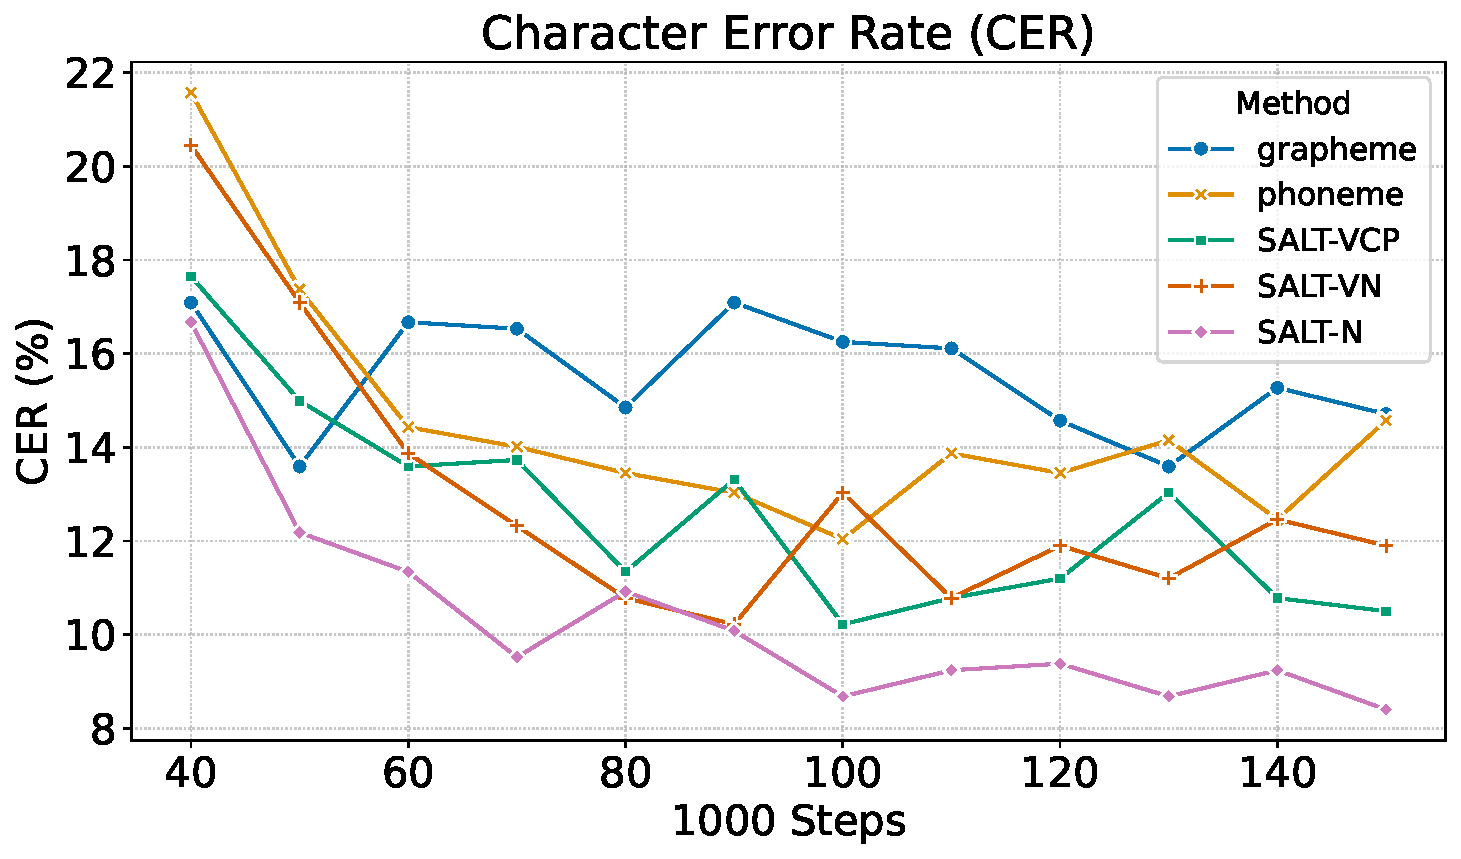
\includegraphics[width=0.92\textwidth]{figures/1h_CER.pdf}
\caption{1시간 저자원 환경에서의 validation CER~\cite{kim2026salt}.
PDF 등 벡터 이미지를 권장합니다.}
\label{fig:cer}
\end{figure}

\texttt{\textbackslash begin\{figure\}}의 위치 지정자로는
\texttt{h}(여기), \texttt{t}(위), \texttt{b}(아래), \texttt{p}(단독 페이지),
\texttt{!}(강제에 가깝게)를 조합할 수 있습니다.

\section{수식}

인라인 수식은 \texttt{\$ ... \$}로 작성합니다. 예: $\alpha = 2.5$.
독립 수식은 \texttt{align} 등을 사용합니다.

\begin{align}
\label{eq:example}
H_{\alpha}(X)
&= \frac{1}{1-\alpha}\log\sum_{i} p_{i}^{\alpha}, \\
\eta_{\alpha}(X)
&= \frac{H_{\alpha}(X)}{\log |V|}.
\end{align}

식~\eqref{eq:example}과 같이 \texttt{\textbackslash eqref}로 참조합니다.

\section{문헌 인용 유형 예시}

\texttt{mybib.bib}에는 유형별 샘플이 들어 있습니다.
본문에서는 각 유형을 한 번씩 인용해 두면 서식 차이를 확인하기 쉽습니다.

\begin{itemize}
    \item 단행본(\texttt{@book}):~\cite{shin2012sounds}
    \item 학술지(\texttt{@article}):~\cite{chen2022wavlm}
    \item 학회(\texttt{@inproceedings}):~\cite{chen2025f5, hong2008effects}
    \item 미발행 논문 등(\texttt{@unpublished}):~\cite{kim2026salt}
    \item 기타(\texttt{@misc}):~\cite{sogang2025aiswthesisguide}
\end{itemize}

%==============================================================================
\chapter{참고문헌}
%==============================================================================

\section{mybib.bib 사용법}

참고문헌은 \texttt{mybib.bib}에 BibTeX 항목으로 관리합니다.
본문에서는 \texttt{\textbackslash cite\{키\}}로 인용하고,
문서 끝에 \texttt{\textbackslash bibliography\{mybib\}}를 둡니다.

학회 등에서 채택되었으나 출판 전이라 proceedings가 아직 없는 논문 등은
\texttt{@unpublished}에 \texttt{note=\{Accepted to ..., to appear\}}를 적습니다.
proceedings가 공개되면 \texttt{@inproceedings}로 바꾸고
\texttt{booktitle}, \texttt{pages} 등을 채우시면 됩니다.

웹페이지·공지사항·소프트웨어 등은 \texttt{@misc}와
\texttt{howpublished}, \texttt{note} 등을 사용합니다.
예: 학위논문작성지침 공지~\cite{sogang2025aiswthesisguide}.

참고문헌 목록은 본문 인용 순으로 정렬됩니다(\texttt{aisw.bst} = unsrt 계열).
지침의 상계서·Ibid./op.~cit. 등 재인용 표기는 BibTeX가 자동으로 처리하지 않으므로,
필요하면 각주(\texttt{\textbackslash footnote})로 작성하시기 바랍니다.
참고문헌과 각주는 구분하여, 참고문헌은 본문 끝에 일괄 기재하고
각주는 해당 페이지 하단에 둡니다.

\section{마무리 점검}

제출 전에 다음을 확인하시기 바랍니다.
\begin{enumerate}
    \item 국문·영문 제목, 저자명(띄어쓰기·붙여쓰기), 지도교수·심사위원
    \item 제출일·심사일·졸업일
    \item 초록 키워드
    \item 표·그림 캡션과 본문 참조
    \item \texttt{pdflatex}--\texttt{bibtex}--\texttt{pdflatex}--\texttt{pdflatex} 후 인용 번호
    \item 더미 예시(김석사, 20XX 등)가 남아 있지 않은지
\end{enumerate}

\bibliography{mybib}

\end{document}
